\section{Emcee Method}

We can also obtain random deviates from any distribution by using Emcee method. The implementation is described in problem 7 noting the following:
\begin{itemize}
    \item The posterior probability is given by a sine function. Adding the prior of this probability: for values outside of $(0,\pi)$ is zero.
    \item The walkers were determined from a uniform probability from $[0,\pi]$.
\end{itemize}

For this case, the number of trials was about 100,000 so it will fill the probability space and truly resemble a sine probability function. 

Figure \ref{fig:emceeRandPlot} shows an histogram of the random samples obtained from Emcee alongside the normalized probability distribution described by equation \ref{eq:sinProb}. We can note that the histogram resembles the normalized probability distribution accurately.
 
% Use the emcee python package to draw random deviates from
% a probability distribution shaped like the first half-cycle of a sine function (properly normalized)
% on the interval $[0,\pi]$.

\begin{figure}
    \centering
    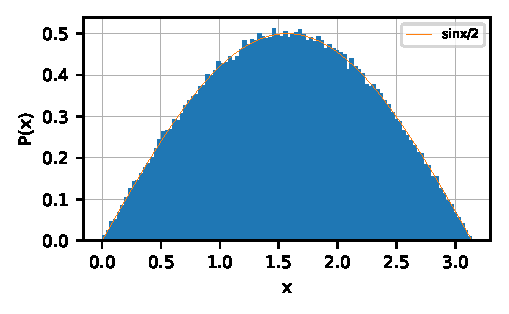
\includegraphics{CodeAndFigures/emceeRandomDeviatesPlot.pdf}
    \caption{Histogram that shows the random deviates obtained from emcee by implementing a sine function as the probability distribution from which the random deviates are from and which should resemble the probability given in equation \ref{eq:sinProb}.}
    \label{fig:emceeRandPlot}
\end{figure}